\documentclass{article}

\usepackage{graphicx}
\usepackage{tikz}
\usepackage{tikzsymbols}
\usetikzlibrary{calc,patterns,shapes.geometric}
\pagestyle{empty}
\usepackage[margin=0pt]{geometry}
\geometry{papersize={14in,12in}}

\def\centerarc[#1](#2)(#3:#4:#5){\draw[#1] ($(#2)+({#5*cos(#3)},{#5*sin(#3)})$) arc (#3:#4:#5);}

\begin{document}
	\begin{figure}
		\centering
		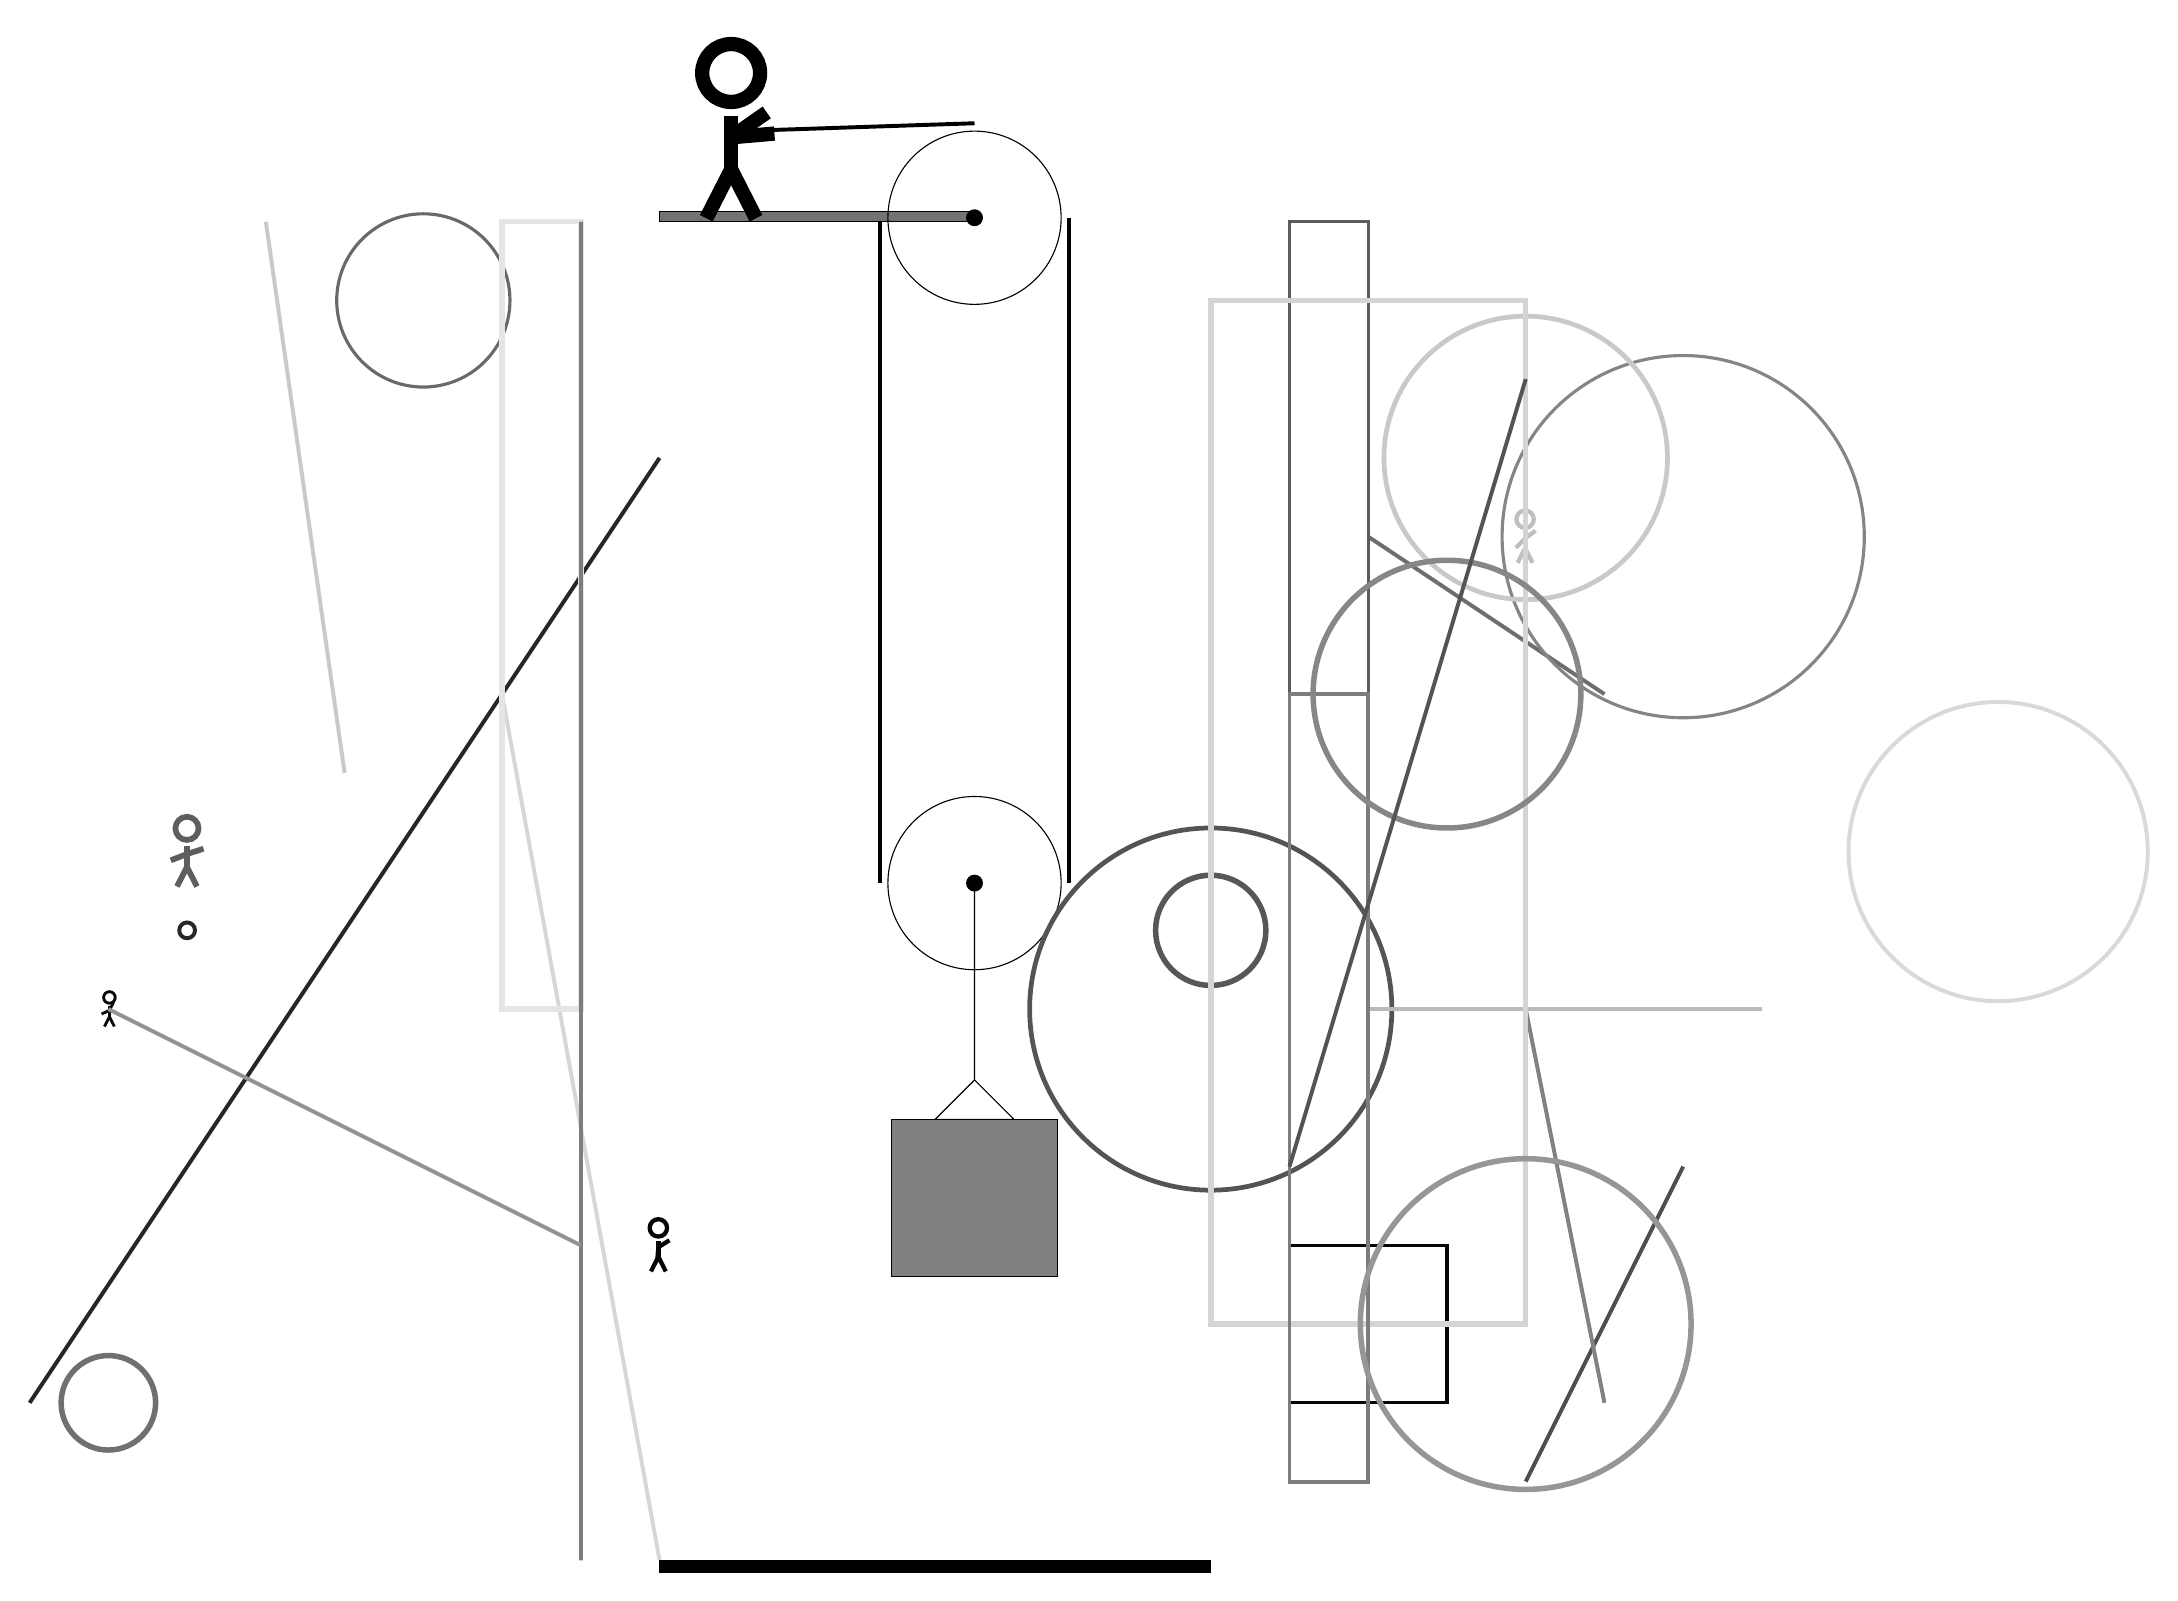
\begin{tikzpicture}
			%%%%% START %%%%%
			
			\draw[fill=black!55] (-2, 14) rectangle (2, 14.125);
			
			\draw (2, 5.6) circle (1.1);
			\draw[fill=black] (2, 5.6) circle (0.1);
			
			\draw[line width=0.5mm, color=black!57](7, 10) -- (10, 8);
			
			\node[line width=0.2mm, color=black!25] at (9, 10) {\Strichmaxerl[3][45][37]};
			\draw[line width=0.5mm, color=black!69](9, -2) -- (11, 2);
			\draw [line width=0.5mm, color=black!85](-8, 5) circle (0.1);
			\draw [line width=0.4mm, color=black!59](-5, 13) circle (1.1);
			
			\draw [line width=0.7mm, color=black!56](-9, -1) circle (0.6);
			\draw[line width=0.5mm, color=black!16](-2, -3) -- (-4, 8);
			
			\draw[line width=0.4mm, color=black!64] (7, 14) rectangle (6, -2);
			\draw [line width=0.4mm, color=black!48](11, 10) circle (2.3);
			\draw[line width=0.2mm, color=black!59] (6, -1) rectangle (8, 1);
			
			\draw[line width=0.5mm, color=black!49](10, -1) -- (9, 4);
			
			\node[line width=0.6mm, color=black!97] at (-9, 4) {\Strichmaxerl[2][25][63]};
			\draw[line width=0.5mm, color=black!85](-2, 11) -- (-10, -1);
			
			\draw[line width=0.4mm, color=black!98] (6, 1) rectangle (8, -1);
			\draw [line width=0.6mm, color=black!67](5, 4) circle (2.3);
			\node[line width=0.3mm, color=black!98] at (-2, 1) {\Strichmaxerl[3][85][32]};
			
			\draw[line width=0.7mm, color=black!10] (-3, 4) rectangle (-4, 14);
			\draw [line width=0.7mm, color=black!66](5, 5) circle (0.7);
			\draw[line width=0.5mm, color=black!27](7, 4) -- (12, 4);
			\draw [line width=0.6mm, color=black!21](9, 11) circle (1.8);
			\draw[line width=0.7mm, color=black!17] (5, 13) rectangle (9, 0);
			\draw[line width=0.5mm, color=black!51] (-3, -3) rectangle (-3, 14);
			\draw[line width=0.5mm, color=black!51] (7, -2) rectangle (6, 8);
			\draw[line width=0.5mm, color=black!21](-7, 14) -- (-6, 7);
			\draw [line width=0.5mm, color=black!15](15, 6) circle (1.9);
			\draw [line width=0.7mm, color=black!47](8, 8) circle (1.7);
			\draw [line width=0.7mm, color=black!41](9, 0) circle (2.1);
			\draw[line width=0.5mm, color=black!42](-3, 1) -- (-9, 4);
			\node[line width=0.5mm, color=black!63] at (-8, 6) {\Strichmaxerl[4][21][18]};
			\draw[line width=0.5mm, color=black!67](6, 2) -- (9, 12);
			
			\draw (2, 14.05) circle (1.1);
			\draw[fill=black] (2, 14.05) circle (0.1);
			
			\draw (2, 5.6) -- (2, 3.1) -- (1.5, 2.6) -- (2.5, 2.6) -- (2, 3.1);
			\draw[fill=black!50] (0.95, 2.6) rectangle (3.05, 0.6);
			
			\draw[line width=0.5mm] (0.8, 14) -- (0.8, 5.6);
			\centerarc[line width=0.5mm](2, 5.6)(180:360:1.2000000000000002);
			\draw[line width=0.5mm](3.2, 5.6) -- (3.2, 14.05);
			\centerarc[line width=0.5mm](2, 14.05)(0:90:1.2000000000000002);
			\draw[line width=0.5mm](2, 15.25) -- (-1, 15.15);
			
			\node at (-1, 15.15) {\Strichmaxerl[10][-175][35]};
			
			\draw[fill=black] (-2, -3) rectangle (5, -3.15);
			
			%%%%% END %%%%%
		\end{tikzpicture}
	\end{figure}	
\end{document}